\documentclass{article}
\usepackage[utf8]{inputenc}
%%%%%%%%% options for the file macros.tex

\def\showauthornotes{1}
\def\showkeys{0}
\def\showdraftbox{0}
\let\pref=\prettyref


%% Shamelessly adapted from a scribe template by Sanjeev Arora

%%%%%%%%%%%%%% Packages
% \usepackage[active,tightpage]{preview}
% \renewcommand{\PreviewBorder}{1in}
\usepackage{hyperref}
\usepackage{amsmath,amssymb,amsthm,amstext,amsfonts,bbm,algorithm,algorithmicx,xspace,nicefrac,
  algpseudocode}
\usepackage{color,stmaryrd,enumerate,latexsym,bm,amsfonts,
  subfigure,wrapfig,verbatim,tabularx,textcomp}
\usepackage[small]{caption}
\usepackage{comment} 
\usepackage{epsfig} 
\usepackage{latexsym,nicefrac,bbm}
\usepackage{xspace}
\usepackage{color,fancybox,graphicx,url,subfigure}
\usepackage{enumitem, fullpage}
\usepackage{booktabs}
\usepackage{commath}
\usepackage{mdframed}
\usepackage{pdfsync}
\usepackage{tikz}
\usetikzlibrary {positioning}

%%%%%%%%%%%%%% Use for definitions
\newcommand{\defeq}{\stackrel{\textup{def}}{=}}

%%%%%%%%%%%%%% Theorem Environments
\newtheorem{theorem}{Theorem}[section]
\newtheorem{problem}[theorem]{Problem}
\newtheorem{lemma}[theorem]{Lemma}
\newtheorem{definition}[theorem]{Definition}
\newtheorem{corollary}[theorem]{Corollary}
\newtheorem{conjecture}[theorem]{Conjecture}
\newtheorem{proposition}[theorem]{Proposition}
\newtheorem{fact}[theorem]{Fact}
\newtheorem{remark}[theorem]{Remark}

%%%%%%%%%%%%%% Probability stuff
\DeclareMathOperator*{\pr}{\bf Pr}
\DeclareMathOperator*{\av}{\mathbbm{E}}
\DeclareMathOperator*{\var}{\bf Var}

%%%%%%%%%%%%%% Matrix stuff
\newcommand{\tr}[1]{\mathop{\mbox{Tr}}\left({#1}\right)}
\newcommand{\diag}[1]{{\bf Diag}\left({#1}\right)}

%% Notation for integers, natural numbers, reals, fractions, sets, cardinalities
%%and so on
\newcommand{\nfrac}[2]{\nicefrac{#1}{#2}}
\def\abs#1{\left| #1 \right|}
\renewcommand{\norm}[1]{\ensuremath{\left\lVert #1 \right\rVert}}

\newcommand{\floor}[1]{\left\lfloor\, {#1}\,\right\rfloor}
\newcommand{\ceil}[1]{\left\lceil\, {#1}\,\right\rceil}

\newcommand{\pair}[1]{\left\langle{#1}\right\rangle} %for inner product

\newcommand\B{\{0,1\}}      % boolean alphabet  use in math mode
\newcommand\bz{\mathbb Z}
\newcommand\nat{\mathbb N}
\newcommand\rea{\mathbb R}
\newcommand\com{\mathbb{C}}
\newcommand\plusminus{\{\pm 1\}}
\newcommand\Bs{\{0,1\}^*}   % B star use in math mode
\newcommand{\ones}{\mathbbm{1}}
\newcommand{\eye}{\mathbbm{I}}



\newcommand{\V}[1]{\mathbf{#1}\ignorespaces}
\renewcommand\AA{\boldsymbol{\mathit{A}}}
\newcommand\LL{\boldsymbol{\mathit{L}}}

% Used to denote bold commands
                                % e.g. vectors, matrices
\DeclareRobustCommand{\fracp}[2]{{#1 \overwithdelims()#2}}
\DeclareRobustCommand{\fracb}[2]{{#1 \overwithdelims[]#2}}
\newcommand{\marginlabel}[1]%
{\mbox{}\marginpar{\it{\raggedleft\hspace{0pt}#1}}}
\newcommand\card[1]{\left| #1 \right|} %cardinality of set S; usage \card{S}
\renewcommand\set[1]{\left\{#1\right\}} %usage \set{1,2,3,,}
\renewcommand\complement{\ensuremath{\mathsf{c}}}
\newcommand\poly{\mbox{poly}}  %usage \poly(n)
\newcommand{\comp}[1]{\overline{#1}}
\newcommand{\smallpair}[1]{\langle{#1}\rangle}
\newcommand{\ol}[1]{\ensuremath{\overline{#1}}\xspace}
\newcommand{\eps}{\epsilon}
\DeclareMathOperator{\vol}{\mathsf{vol}}


%%%%%%%%%%%%%% Mathcal shortcuts
\newcommand\calF{\mathcal{F}}
\newcommand\calP{\mathcal{P}}
\newcommand\calS{\mathcal{S}}
\newcommand\calG{\mathcal{G}}
\newcommand\calH{\mathcal{H}}
\newcommand\calC{\mathcal{C}}
\newcommand\calD{\mathcal{D}}
\newcommand\calI{\mathcal{I}}
\newcommand\calV{\mathcal{V}}
\newcommand\calK{\mathcal{K}}
\newcommand\calN{\mathcal{N}}
\newcommand\calX{\mathcal{X}}
\newcommand\calU{\mathcal{U}}
\newcommand\calE{\mathcal{E}}

%%%%%%%%%%%%%% {{{ authornotes }}}
\definecolor{Mygray}{gray}{0.8}

 \ifcsname ifcommentflag\endcsname\else
  \expandafter\let\csname ifcommentflag\expandafter\endcsname
                  \csname iffalse\endcsname
\fi

\ifnum\showauthornotes=1
\newcommand{\todo}[1]{\colorbox{Mygray}{\color{red}#1}}
\else
\newcommand{\todo}[1]{#1}
\fi

\ifnum\showauthornotes=1
\newcommand{\Authornote}[2]{{\sf\small\color{red}{[#1: #2]}}}
\newcommand{\Authoredit}[2]{{\sf\small\color{red}{[#1]}\color{blue}{#2}}}
\newcommand{\Authorcomment}[2]{{\sf \small\color{gray}{[#1: #2]}}}
\newcommand{\Authorfnote}[2]{\footnote{\color{red}{#1: #2}}}
\newcommand{\Authorfixme}[1]{\Authornote{#1}{\textbf{??}}}
\newcommand{\Authormarginmark}[1]{\marginpar{\textcolor{red}{\fbox{%\Large
#1:!}}}}
\else
\newcommand{\Authornote}[2]{}
\newcommand{\Authoredit}[2]{}
\newcommand{\Authorcomment}[2]{}
\newcommand{\Authorfnote}[2]{}
\newcommand{\Authorfixme}[1]{}
\newcommand{\Authormarginmark}[1]{}
\fi


%%%%%%%%%%%%%% Logical operators
\newcommand\true{\mbox{\sc True}}
\newcommand\false{\mbox{\sc False}}
\def\scand{\mbox{\sc and}}
\def\scor{\mbox{\sc or}}
\def\scnot{\mbox{\sc not}}
\def\scyes{\mbox{\sc yes}}
\def\scno{\mbox{\sc no}}

%% Parantheses
\newcommand{\paren}[1]{\unskip\left({#1}\right)}
\newcommand{\sqparen}[1]{\unskip\left[{#1}\right]}
\newcommand{\curlyparen}[1]{\unskip\left\{{#1}\right\}}
\newcommand{\smallparen}[1]{\unskip({#1})}
\newcommand{\smallsqparen}[1]{\unskip[{#1}]}
\newcommand{\smallcurlyparen}[1]{\unskip\{{#1}\}}

%% short-hands for relational simbols

\newcommand{\from}{:}
\newcommand\xor{\oplus}
\newcommand\bigxor{\bigoplus}
\newcommand{\logred}{\leq_{\log}}
\def\iff{\Leftrightarrow}
\def\implies{\Rightarrow}




%% macros to write pseudo-code

\newlength{\pgmtab}  %  \pgmtab is the width of each tab in the
\setlength{\pgmtab}{1em}  %  program environment
 \newenvironment{program}{\renewcommand{\baselinestretch}{1}%
\begin{tabbing}\hspace{0em}\=\hspace{0em}\=%
\hspace{\pgmtab}\=\hspace{\pgmtab}\=\hspace{\pgmtab}\=\hspace{\pgmtab}\=%
\hspace{\pgmtab}\=\hspace{\pgmtab}\=\hspace{\pgmtab}\=\hspace{\pgmtab}\=%
\+\+\kill}{\end{tabbing}\renewcommand{\baselinestretch}{\intl}}
\newcommand {\BEGIN}{{\bf begin\ }}
\newcommand {\ELSE}{{\bf else\ }}
\newcommand {\IF}{{\bf if\ }}
\newcommand {\FOR}{{\bf for\ }}
\newcommand {\TO}{{\bf to\ }}
\newcommand {\DO}{{\bf do\ }}
\newcommand {\WHILE}{{\bf while\ }}
\newcommand {\ACCEPT}{{\bf accept}}
\newcommand {\REJECT}{\mbox{\bf reject}}
\newcommand {\THEN}{\mbox{\bf then\ }}
\newcommand {\END}{{\bf end}}
\newcommand {\RETURN}{\mbox{\bf return\ }}
\newcommand {\HALT}{\mbox{\bf halt}}
\newcommand {\REPEAT}{\mbox{\bf repeat\ }}
\newcommand {\UNTIL}{\mbox{\bf until\ }}
\newcommand {\TRUE}{\mbox{\bf true\ }}
\newcommand {\FALSE}{\mbox{\bf false\ }}
\newcommand {\FORALL}{\mbox{\bf for all\ }}
\newcommand {\DOWNTO}{\mbox{\bf down to\ }}

% Theorem-type environments
% \theoremstyle{break} 
% \theoremheaderfont{\scshape}
% \theorembodyfont{\slshape}
% \newtheorem{Thm}{Theorem}[section]
% \newtheorem{Lem}[Thm]{Lemma}
% \newtheorem{Cor}[Thm]{Corollary}
% \newtheorem{Prop}[Thm]{Proposition}
% % \theoremstyle{plain} 
% % \theorembodyfont{\rmfamily} 
% \newtheorem{Ex}[Thm]{Exercise}
% \newtheorem{Exa}[Thm]{Example}
% \newtheorem{Rem}[Thm]{Remark}
% % \theorembodyfont{\itshape}
% \newtheorem{Def}[Thm]{Definition}
% \newtheorem{Conj}[Thm]{Conjecture}
% \newtheorem{Obs}[Thm]{Observation}
% \newtheorem{Ques}[Thm]{Question}
%\newenvironment{proof}{\noindent {\sc Proof:}}{$\Box$ \medskip} 
\newenvironment{problems} % Definition of problems
 {\renewcommand{\labelenumi}{\S\theenumi}
	\begin{enumerate}}{\end{enumerate}}


%%%%%%%%%%%%%%%%% Proof Environments

\def\FullBox{\hbox{\vrule width 6pt height 6pt depth 0pt}}
%
%\def\qed{\ifmmode\qquad\FullBox\else{\unskip\nobreak\hfil
%\penalty50\hskip1em\null\nobreak\hfil\FullBox
%\parfillskip=0pt\finalhyphendemerits=0\endgraf}\fi}

\def\qedsketch{\ifmmode\Box\else{\unskip\nobreak\hfil
\penalty50\hskip1em\null\nobreak\hfil$\Box$
\parfillskip=0pt\finalhyphendemerits=0\endgraf}\fi}

%\newenvironment{proof}{\begin{trivlist} \item {\bf Proof:~~}}
 %  {\qed\end{trivlist}}

\newenvironment{proofsketch}{\begin{trivlist} \item {\bf
Proof Sketch:~~}}
  {\qedsketch\end{trivlist}}

\newenvironment{proofof}[1]{\begin{trivlist} \item {\bf Proof
#1:~~}}
  {\qed\end{trivlist}}

\newenvironment{claimproof}{\begin{quotation} \noindent
{\bf Proof of claim:~~}}{\qedsketch\end{quotation}}


%%%%%%%%%%%%%%%%%%%%%%%%%%%%%%%%%%%%%%%%%%%%%%%%%%%%%%%%%%%%%%%%%%%%%%%%%%%
%%%%%%%%%%%%%%%%%%%%%%%%%%%%%%%%%%%%%%%%%%%%%%%%%%%%%%%%%%%%%%%%%%%%%%%%%%%




\newlength{\tpush}
\setlength{\tpush}{2\headheight}
\addtolength{\tpush}{\headsep}

\newcommand{\handout}[5]{
   \noindent
   \begin{center}
   \framebox{ \vbox{ \hbox to \textwidth { {\bf \coursenum\ :\  \coursename} \hfill #5 }
       \vspace{3mm}
       \hbox to \textwidth { {\Large \hfill #2  \hfill} }
       \vspace{1mm}
       \hbox to \textwidth { {\it #3 \hfill #4} }
     }
   }
   \end{center}
   \vspace*{4mm}
   \newcommand{\lecturenum}{#1}
   \addcontentsline{toc}{chapter}{Lecture #1 -- #2}
}

\newcommand{\lecturetitle}[4]{\handout{#1}{#2}{Lecturer: \courseprof
  }{Scribe: #3}{Lecture #1 : #4}}
\newcommand{\guestlecturetitle}[5]{\handout{#1}{#2}{Lecturer:
    #4}{Scribe: #3}{Lecture #1 - #5}}


%%%%%%%%%%%%%%%%%%%%%%%%%%%%%%%%%%%%%%%%%%%%%%%%%%%%%%%%%
%%% Commands to include figures


%% PSfigure

\newcommand{\PSfigure}[3]{\begin{figure}[t] 
  \centerline{\vbox to #2 {\vfil \psfig{figure=#1.eps,height=#2} }} 
  \caption{#3}\label{#1} 
  \end{figure}} 
\newcommand{\twoPSfigures}[5]{\begin{figure*}[t]
  \centerline{%
    \hfil
    \begin{tabular}{c}
        \vbox to #3 {\vfil\psfig{figure=#1.eps,height=#3}} \\ (a)
    \end{tabular}
    \hfil\hfil\hfil
    \begin{tabular}{c}
        \vbox to #3 {\vfil\psfig{figure=#2.eps,height=#3}} \\ (b)
    \end{tabular}
    \hfil}
  \caption{#4}
  \label{#5}
%  \sublabel{#1}{(a)}
%  \sublabel{#2}{(b)}
  \end{figure*}}

\newcounter{fignum}

% fig
%command to insert figure. usage \fig{name}{h}{caption}
%where name.eps is the postscript file and h is the height in inches
%The figure is can be referred to using \ref{name}
\newcommand{\fig}[3]{%
\begin{minipage}{\textwidth}
\centering\epsfig{file=#1.eps,height=#2}
\caption{#3} \label{#1}
\end{minipage}
}%


% ffigure
% Usage: \ffigure{name of file}{height}{caption}{label}
\newcommand{\ffigure}[4]{\begin{figure} 
  \centerline{\vbox to #2 {\hfil \psfig{figure=#1.eps,height=#2} }} 
  \caption{#3}\label{#4} 
  \end{figure}} 

% ffigureh
% Usage: \ffigureh{name of file}{height}{caption}{label}
\newcommand{\ffigureh}[4]{\begin{figure}[!h] 
  \centerline{\vbox to #2 {\vfil \psfig{figure=#1.eps,height=#2} }} 
  \caption{#3}\label{#4} 
  \end{figure}} 


% {{{ draftbox }}}
\ifnum\showdraftbox=1
\newcommand{\draftbox}{\begin{center}
  \fbox{%
    \begin{minipage}{2in}%
      \begin{center}%
%        \begin{Large}%
          \large\textsc{Working Draft}\\%
%        \end{Large}\\
        Please do not distribute%
      \end{center}%
    \end{minipage}%
  }%
\end{center}
\vspace{0.2cm}}
\else
\newcommand{\draftbox}{}
\fi


%% Complexity classes
\newcommand\p{\mbox{\bf P}\xspace}
\newcommand\np{\mbox{\bf NP}\xspace}
\newcommand\cnp{\mbox{\bf coNP}\xspace}
\newcommand\sigmatwo{\mbox{\bf $\Sigma_2$}\xspace}
\newcommand\ppoly{\mbox{\bf $\p_{\bf /poly}$}\xspace}
\newcommand\sigmathree{\mbox{\bf $\Sigma_3$}\xspace}
\newcommand\pitwo{\mbox{\bf $\Pi_2$}\xspace}
\newcommand\rp{\mbox{\bf RP}\xspace}
\newcommand\zpp{\mbox{\bf ZPP}\xspace}
\newcommand\bpp{\mbox{\bf BPP}\xspace}
\newcommand\ph{\mbox{\bf PH}\xspace}
\newcommand\pspace{\mbox{\bf PSPACE}\xspace}
\newcommand\npspace{\mbox{\bf NPSPACE}\xspace}
\newcommand\dl{\mbox{\bf L}\xspace}
\newcommand\ma{\mbox{\bf MA}\xspace}
\newcommand\am{\mbox{\bf AM}\xspace}
\newcommand\nl{\mbox{\bf NL}\xspace}
\newcommand\conl{\mbox{\bf coNL}\xspace}
\newcommand\sharpp{\mbox{\#{\bf P}}\xspace}
\newcommand\parityp{\mbox{$\oplus$ {\bf P}}\xspace}
\newcommand\ip{\mbox{\bf IP}\xspace}
\newcommand\pcp{\mbox{\bf PCP}}
\newcommand\dtime{\mbox{\bf DTIME}}
\newcommand\ntime{\mbox{\bf NTIME}}
\newcommand\dspace{\mbox{\bf SPACE}\xspace}
\newcommand\nspace{\mbox{\bf NSPACE}\xspace}
\newcommand\cnspace{\mbox{\bf coNSPACE}\xspace}
\newcommand\exptime{\mbox{\bf EXP}\xspace}
\newcommand\nexptime{\mbox{\bf NEXP}\xspace}
\newcommand\genclass{\mbox{$\cal C$}\xspace}
\newcommand\cogenclass{\mbox{\bf co$\cal C$}\xspace}
\newcommand\size{\mbox{\bf SIZE}\xspace}
\newcommand\sig{\mathbf \Sigma}
\newcommand\pip{\mathbf \Pi}

%%Computational problems
\newcommand\sat{\mbox{SAT}\xspace}
\newcommand\tsat{\mbox{3SAT}\xspace}
\newcommand\tqbf{\mbox{TQBF}\xspace}


%%%%%%%%% Authornotes
\newcommand{\Snote}{\Authornote{S}}
\newcommand{\Scomment}{\Authorcomment{S}}
\newcommand{\Sfnote}{\Authorfnote{S}}


\title{CSC2240 Class Project -- Oblivious Subspace Embeddings}
\author{Aida Ramezani \& Marc-Etienne Brunet}
\date{November 2022}

\usepackage[a4paper, total={4in, 8in}]{geometry}
\begin{document}



\maketitle

\section{Introduction}
\subsection{Outline}
\begin{enumerate}
    \item [{[}3 min{]}] What are subspace embeddings? Compare to JL lemma.
    \item [{[}3 min{]}] Why are they interesting? Motivate with regression, compare to JL lemma. 
    \item [{[}3 min{]}] Why do we want sparse subspace embeddings?
    \item [{[}11 min{]}] Sketch the simpler Matrix-Chernoff bounds from Section ``Our Approach''.
    \item [{[}5 min{]}] Demo - either regression or NLP. 
    \item [{[}5 min{]}] Q \& A
\end{enumerate}

\subsection{Notation}
\begin{tabular}{c|l}
    $n$ & dimension in original space \\
    $m$ & dimension of embedding \\
    $\Pi$ & embedding matrix $\in \rea^{m \times n}$ \\
    $k$ & number of vectors preserved by JL \\
    $d$ & dimension of subspace \\
\end{tabular}

\subsection{What are oblivious subspace embeddings (OSEs)?}
Similar to the JL-Lemma, 
oblivious subspace embeddings (OSEs), are  oblivious, $\epsilon$-distortion, random embeddings.
However, rather than just embedding a finite set of $k$ vectors,
they are concerned with embedding an entire $d$-dimensional subspace. 
In the main work that we covered, \cite{cohen2016nearly}, OSEs are defined as follows:
%
\begin{definition}[Oblivious Subspace Embedding]
    A probability distribution over $m$ by $n$ matrices, $\Pi$,
    is defined to be a $(d, \epsilon, \delta)$-OSE if,
    for any $d$-dimensional subspace $S$ of $\rea^n$,
    \begin{align}
        \pr \left[ \left( \max_{\xx \in S, \norm{x}=1} \left| \norm{\Pi\xx}^2 - 1\right| \right) > \epsilon \right] < \delta.
    \end{align}
\end{definition}
%
From what we've found, 
the extension of the JL-Lemma to subspaces was originally done by~\cite{sarlos2006improved},
who showed that a $d$-dimensional \textit{subspace} of $\rea^n$,
could be embedded into $m=\calO(\epsilon^{-2}d\log(d/\epsilon))$ dimensions
and similarly approximately preserve the lengths of all vectors in the subspace.
The allowable distortion is visualized in Figure~\ref{fig:distortion_and_net} (left).
%
\begin{lemma}
\label{lem:subspace_ext}
Let $S$ be an arbitrary d dimensional subspace of $\rea^n$ and $\epsilon \in (0, 1/2]$, $\delta < 1$. 
If $\Pi$ is a JL transform from $\rea^n$ to 
$m=\calO(\epsilon^{-2}d\log(d/\epsilon) \cdot f(\delta))$ dimensions for some 
function f, then
\begin{align*}
    \pr \left[ \forall \xx \in S~~(1-\epsilon) \norm{\xx} \leq \norm{\Pi\xx} \leq (1+\epsilon)\norm{\xx} \right]
            \geq 1-\delta.
\end{align*}
\end{lemma}
%
\begin{proofsketch}
The key idea of the proof is then to cover the unit sphere with an epsilon-net 
that is sufficiently fine that every $\xx \in S$ is close enough to a point in the net.
This is visualized in Figure~\ref{fig:distortion_and_net}(right).
The epsilon net used in the proof has $\calO((k/\epsilon)^k)$ elements.
Plugging that many elements into the union bound used to prove \ref{thm:jl_lemma},
in place of $\binom{k}{2}$, we get to the stated complexity. 
For more details, see Lemma 10 in \cite{sarlos2006improved}.
\end{proofsketch}
%
\begin{figure}
    \centering
    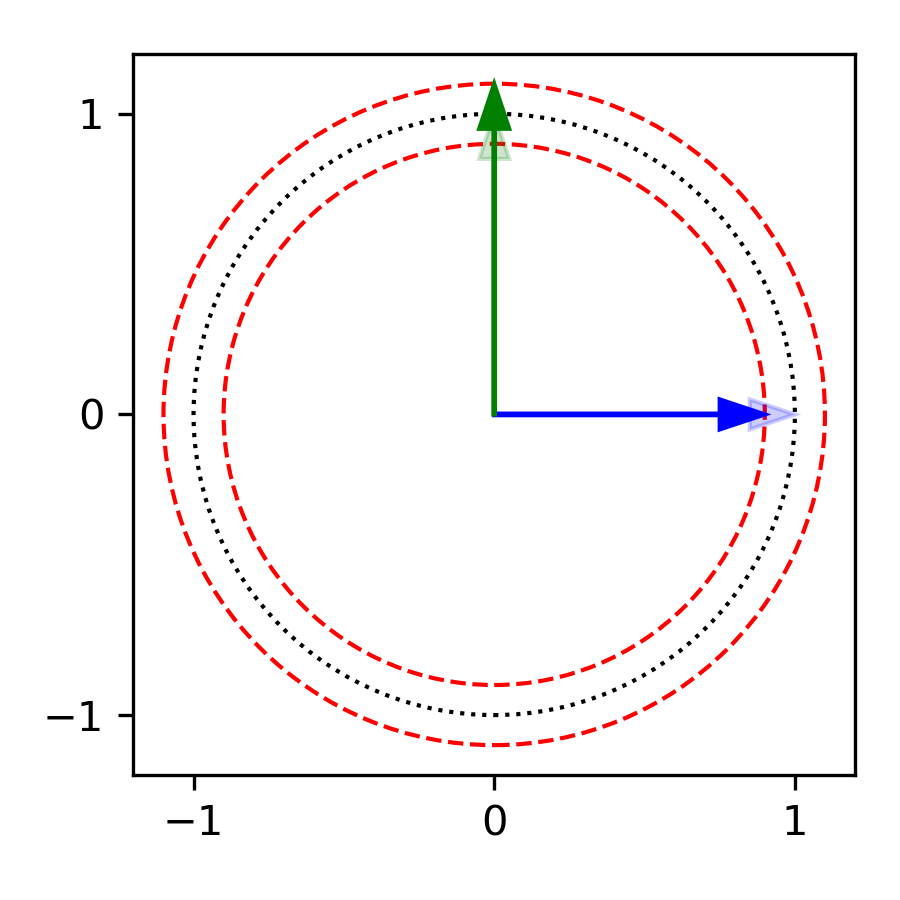
\includegraphics{figures/unit_sphere.png}
    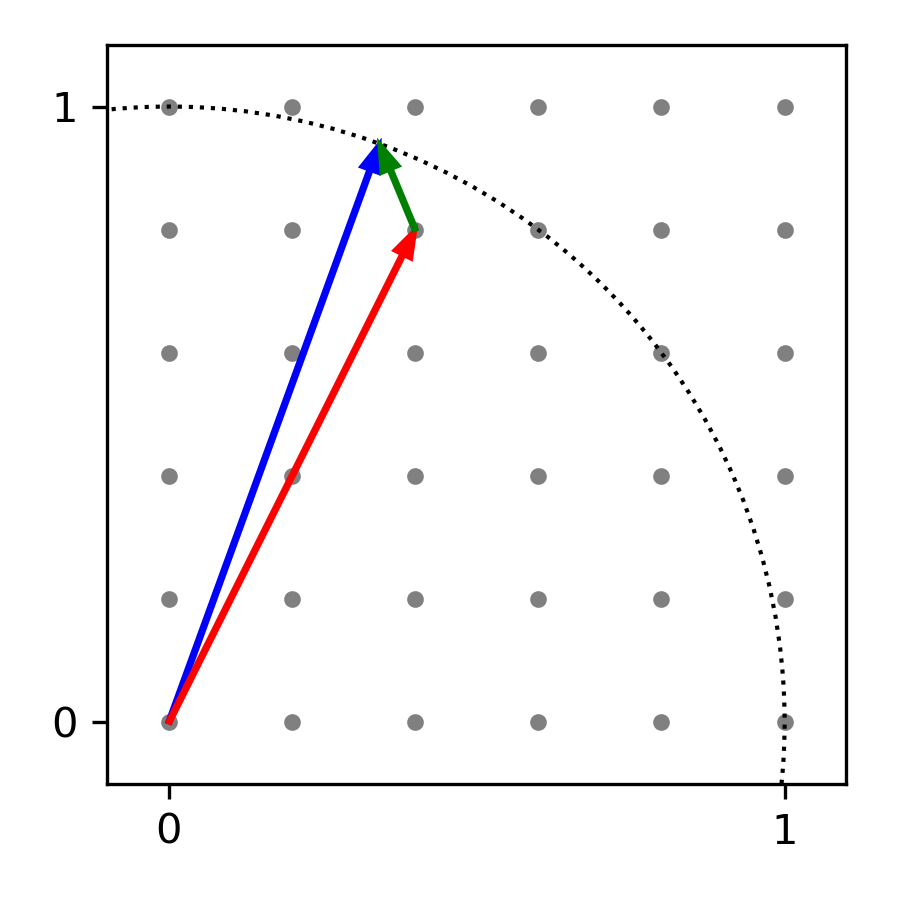
\includegraphics{figures/epsilon_net.png}
    \caption{Left – Visualization of allowable distortion vectors in the preserved subspace $S$. 
    Unit vectors must not be distorted out of the $\pm \epsilon$ shell. 
    Right – Visualization of the epsilon net used to prove Lemma~\ref{lem:subspace_ext}. 
    The blue vector is an arbitary vector on the unit sphere. 
    Using the triangle inequality, its magnitude is less than the sum of the red and green vectors.
    Bounding the distortion of the red vector is easy,
    since it is an element of the net. 
    The distortion of the green vector requires a little more work, 
    but with a sufficiently fine net, this component is very small,
    and the sum of their distortions are shown to be within the $(1\pm \epsilon)$ tolerance. 
    }
    \label{fig:distortion_and_net}
\end{figure}



\subsection{Why are subspace embeddings useful?}
Consider linear regression. We want to find a vector $w^* \in \rea^d$ such that 
\begin{align}
    w^* =  \argmin \norm{Aw - b}^2.
\end{align}
With $A \in \rea^{n \times d}$ being the data matrix (n observations of $d$ features), 
and $n \ggreater d$.
The solution has a closed form expression, 
$w^* = (A^TA)^{-1}(A^Tb)$. 
This solution requires roughly
$\calO(nd^2)$ time for the $A^TA$ multiplication,
$\calO(nd)$ time for the $A^Tb$ multiplication,
and $\calO(d^3)$ time to solve the remaining linear system. 
% Discussion \href{https://math.stackexchange.com/questions/84495/computational-complexity-of-least-square-regression-operation}{here}.

Since we assume $n \ggreater d$, this is dominated by $\calO(nd^2)$.
It would therefore be very interesting to reduce $n$ in $A$,
at the expense of obtaining an inexact solution $\tilde{w}$,
so long as we could bound the relative error of the approximation.
An obvious way to reduce $n$ is to simply sub-sample the rows of $A$, i.e., 
the observations.
But it is unclear whether we can sub-sample those rows with guarantees on the error 
any faster than just solving the original problem \cite{sarlos2006improved}.


\subsection{Why do we want \textit{sparse} subspace embeddings?}
At a high level, we are interested in a sparse subspace embeddings,
because the procedure for sampling a dense embedding matrix $L$,
then multiplying it through to embed the problem, 
may offset the computational benefit of embedding the problem in the first place. 
% What do we mean by sparse?
% How can sparsity further help improve time complexity?
At a high level, we are interested in sparse subspace embeddings because the procedure for sampling a dense embedding matrix $\Pi$, then multiplying it through to embed the problem, 
may offset the computational benefit of embedding the problem in the first place. 

For example, remember that in the Least Squares Regression problem, using subspace embedding matrix $\Pi \in \rea^{m \times n}$, reduces the dimension to $\calO({m d ^2})$. If we use a dense Gaussian matrix from JL-lemma of dimension $\calO(\epsilon ^ {-2}d\log(d))$ for $\Pi$, it would still take $\calO({n d^2 \log(d)})$ to compute $\Pi A$. Therefore, if $n \ggreater d$, our running time is still dominated by $n$, which counteracts the computational benefit of solving the linear system in a smaller dimension. 


We can speed up this process by working with a \textbf{sparse} random matrix $\Pi$. Such matrix would have exactly $s$ non-zero entries on each column. Multiplying $\Pi$ by any matrix, such as $A \in \rea^{n \times d}$, takes $\calO(snd)$ time. If $A$ is also a sparse matrix, it would only take $\calO(s \times Non-zero(A))$ to compute $\Pi A$, where $Non-zero(A)$ is the number of non-zero entries in $A$. 

To construct such matrix $\Pi$, one needs to randomly pick $s$ entries per column and set them to $\pm \frac{1}{\sqrt{s}}$, randomly and uniformly as well. The rest of the entries should be zero. In fact, there is a trade-off between the sparsity $s$ and the row count $m$. In the next section, we will show how matrix trace inequalities can give us an almost tight bound for $(d, \epsilon, \delta)$-OSE, where for any $B > 2$
$$m = \calO(\epsilon^{-2}Bd\log(d/\delta))$$ and $$s = \calO(\epsilon^{-1}\log_B(d/\delta)).$$ Note, that here the parameter $B$ controls the trade-off between $s$ and $m$. If $s$ is small, then the time complexity to compute $\Pi A$ depends only on the non-zero entries of the matrix $A$. However, the reduced dimension $m$ could get so large that storing and working with any vector in this dimension becomes inefficient and costly.  

% When $s = 1$, $m = \calO(\epsilon^{-2}d^2/\delta)$. Given the dependence on $d^2$ and $1/\delta$, decreasing the probability of failure, referred to as $\delta$, becomes costly.

% {\color{red} ADD PROOF from~\cite{nelson2013osnap} for sparse matrices}



\subsection{Sketch of proof of bounds}
To construct the matrix $\Pi \in \rea^{m \times n}$ we randomly select $s$ entries on each column to be non-zero and we set them to be $+\frac{1}{\sqrt{s}}$ or $-\frac{1}{\sqrt{s}}$ with equal probabilities. To formalize this we can use two sets of random variables $\delta_{r,i}$ and $\sigma_{r, i}$, where 

$$
 \delta_{r, i} = 
\begin{cases} 
    1 & \Pi_{r, i} \neq 0 \\
    0 & o.w
\end{cases}
$$
and 
$$
P(\sigma_{r, i} = 1) = P(\sigma_{r, i} = -1) = \frac{1}{2}.
$$
Using this notation, we can write the entries in $\Pi$ as $\Pi_{r, i} = \frac{1}{\sqrt{s}} \delta_{r, i} \sigma_{r, i}$, and proceed with the proof. 

The next step is to quantify the subspace embedding distortion error, which we want to bound by $\calO({\epsilon})$. 


\begin{fact}
    The OSE matrix $\Pi$ successfully embeds a subspace $S$ with an orthonormal basis $U$ if and only if 
    \begin{equation}
        \norm{(\Pi U)^T (\Pi U) - U^TU} \leq \epsilon
    \end{equation}
\end{fact}
\begin{proofsketch}


The reader can note that the spectral norm of a symmetric matrix $A$ is its largest eigenvalue, which can be written as $$ \norm{A} = \max_{\norm{e} = 1} {e^T A e}.$$

Therefore, the spectral norm of the symmetric matrix $(\Pi U)^T (\Pi U) - U^TU$ would be 
$$\norm{(\Pi U)^T (\Pi U) - U^TU} = \max_{\norm{e} = 1}{
     e^T ((\Pi U)^T (\Pi U) - U^TU) e }= \max_{\norm{e} = 1}{\norm{\Pi e}^2 - \norm{e}^2}$$

where, $\norm{\Pi e}^2 - \norm{e}^2$ is the distortion error of the subspace embedding, which we want to bound by $\calO({\epsilon})$. \cite{nelson2013osnap} provide an alternative way to think about this problem. It suffices to write $S$ as $$S = \{x : \exists y \in \rea^{d}, x = Uy\}.$$
Then $\Pi$ is an OSE if and only if $\norm{\Pi x} = (1 \pm \epsilon)\norm{x}$ with high probability. Note that $\norm{\Pi x} = \norm{\Pi U y}$, and since $U$ is a unitary matrix it preserves the norm, thus we have $$\norm{\Pi U y} = \norm{\Pi y} = (1 \pm \epsilon) \norm{y}.$$ 
This property is equivalent to having all the singular values of $\Pi U$ in the range of $(1 - \epsilon, 1 + \epsilon)$, meaning that the eigenvalues of $(\Pi U) ^ T (\Pi U)$ would be in the range of  $( (1 - \epsilon) ^ 2, (1 + \epsilon) ^ 2)$. Now since $U^T U = I$, then 
    $$(\Pi U) ^T (\Pi U) = I + ((\Pi U) ^T (\Pi U) - U^T U).$$
Following Weyl's inequality~\cite{nelson2013osnap} we can show that the eigenvalues of $(\Pi U) ^ T (\Pi U)$ are $1 \pm  \norm{(\Pi U)^T (\Pi U) - U^TU}$, which we need them to be in the range of $(-2\epsilon + \epsilon^2 + 1, 2\epsilon + \epsilon ^2 + 1)$. Consequently if $\epsilon$ is small enough, then $\norm{((\Pi U) ^T (\Pi U) - U^T U)} \leq 3 \epsilon = \calO{(\epsilon)}$

\end{proofsketch}

Now, we can continue the proof by reducing the spectral norm  $\norm{(\Pi U)^T (\Pi U) - U^TU}$ and find an upper bond on $m$ and $s$. One possible approach is to decompose $(\Pi U)^T (\Pi U)$ to its rows and use Matrix Chernoff concentration bound.

\begin{theorem}[MATRIX CHERNOFF]
    Let $A_i$ be independent random positive semi-definite matrices satisfying $\av[\sum{A_i}]= I$ and $\norm{A_i} \leq O(\frac{log(d / \delta)}{\epsilon ^ 2})$, then for any $\epsilon < 1$
   $$P(\norm{\sum A_i - I} \leq \epsilon) \geq 1 - \delta.$$
\end{theorem}
   To use the Matrix Chernoff bound, one can write the matrix $(\Pi U) ^ T (\Pi U)$ as the sum of random matrices:
\begin{equation}
    (\Pi U) ^ T (\Pi U) = \sum_{r}(\Pi U)_r (\Pi U)_r^{T}
\end{equation}
However, the norms of these uniform random matrices ($\norm{(\Pi U)_r ^ T (\Pi U)_r} = \norm{(\Pi U)_r}^{2}$) are not bounded, and they are also not independent. To handle this problem, we can  show that  the contribution of the off-diagonal terms in $(\Pi U)^T (\Pi U)$ gives us a set of new random matrices that are equivalent to the OSE error matrix $(\Pi U)^T (\Pi U) - U^TU$:

\begin{align*}
     (\Pi U) ^ T (\Pi U) & = \sum_{r}(\Pi U)_r {(\Pi U)_r}^{T} \\
     & = \frac{1}{s} \sum_{r} (\sum_{i} \delta_{r, i} \sigma_{r, i} u_i) (\sum_{i} \delta_{r, i} \sigma_{r, i} {u_i}^T) \\
     & = \frac{1}{s} \sum_{r} (\sum_{i} \delta_{r, i} u_i u_i ^T ) + (\sum_{i \neq j} \delta_{r, i} \delta_{r, j} \sigma_{r, i} \sigma_{r, j} u_i {u_j}^T) \\
     & \frac{1}{s} (\sum_{i} (\sum_{r} \delta_{r, i}) u_i {u_i}^T) + \frac{1}{s} (\sum_{r} (\sum_{i \neq j} \delta_{r, i} \delta_{r, j} \sigm_{r, i} \sigma_{r, j} u_i {u_j}^T) 
     \\
     & =  U^T U + \frac{1}{s} \sum_r \sum_{i \neq j} \delta_{r, i} \delta_{r, j} \sigma_{r,i} \sigma_{r, j} u_i {u_j}^{T}
\end{align*}

To find a bound on the spectral norm of $(\Pi U)^T (\Pi U) - U^TU$ we only need to find a matrix concentration bound on the contribution of rows in the off-diagonal entries. For each row, we now have to consider the collision incidents only, i.e., when multiple non-zero entries exist in a row of $\Pi$. We refer to these matrices by $Z_r$:
\begin{equation}
    (\Pi U)^T (\Pi U) - U^TU = \frac{1}{s} \sum_r \sum_{i \neq j} \delta_{r, i} \delta_{r, j} \sigma_{r,i} \sigma_{r, j} u_i u_j ^ T = \frac{1}{s} \sum_r {Z_r}.
\end{equation}
Even though the $Z_r$ variables are still not independent, we can use an alternative form of Matrix Chernoff bound with a
requirements on the conditional distribution of each random variable given the previous ones.
\begin{lemma}
\label{lemma_2}
    Let $A = \sum_i A_i$ be a sum of $m$ random symmetric matrices such that for all $i$ and all allowable values $A_1^{'}, A_2^{'}, \dots A_{i - 1}^{'}$,
    $$
        \norm{\av [cA_i | A_1^{'}, A_2^{'}, \dots A_{i - 1}^{'}]} \leq C  
    $$
then, 
$$
\av[\tr{\exp(cA)}] \leq d C^m.
$$
\end{lemma}

\begin{proof}

Define $S_{i}$ as the partial sum of $A_j$ matrices: $S_{i} = \sum_{j = 1}^{i}A_j$. Without loss of generality we can assume $c = 1$, since $cA_i = B_i$, where $B_i$'s are our new random symmetric matrices. Now, for $i > 0$

\begin{align*}
    \av[\tr{\exp(S_i)}] = &\av_{S_{i-1}}[\av_{A_i}[\tr{\exp(A_i + S_{i-1})}]] \\
    \leq & \av_{S_{i-1}}[\av_{A_i}[\tr{\exp(A_i}\exp(S_{i-1}))]] \\
    = & \av_{S_{i-1}}[\tr{\av_{A_i}[\exp(A_i)]\exp(S_{i-1})}] \\
    \leq & \av_{S_{i-1}}[\norm{\av_{A_i}[\exp(A_i)} \tr{\exp(S_{i-1})}] \\
    \leq & C\av[\tr{\exp(S_{i - 1})}]
\end{align*}
The second line is a result of the \textsc{Golden-Thompson} lemma that shows $$\tr{\exp(A + B)} \leq \tr{\exp(A)\exp(B)}.$$ 
The third line follows the linearity of trace and matrix product as $$\av_{S_{i - 1}}[\av_{A_i}[\tr{\exp(S_{i - 1})}]] = \av_{S_{i - 1}}[\tr{\exp(S_{i - 1})}].$$ 
We use the fact that for two positive semi-definite matrices $A$ and $B$, $\tr{A B} \leq \tr{A} \norm{B}$ to get the forth line, and by using lemma~\ref{exp_lemma}, we show that both $\exp(S_{i - 1})$ and $\av_{A_{i}}[\exp(A_i)]$ are positive semi-definite. Since by definition $\exp(0) = I$, then $\av[\tr{\exp(S_0)}] = d$, and, thus $\av[\tr{\exp(A)}] = dC^m$.
\end{proof}


\begin{lemma}
    The exponential of a symmetric matrix $A$ is positive semi-definite.
\label{exp_lemma}
\end{lemma}
\begin{proof}(Of lemma~\ref{exp_lemma})
    We have to show that $\exp(A)$ is positive semi-definite.
        Since $A$ is symmetric it is diagonalizable, and can write it as
        \begin{align*}
            &A  = P D P ^{-1}\\
            &\exp(A) = \sum_{k = 0}^{\infty} \frac{1}{K!} A^k\\
            &\exp(A) = \sum_{k = 0}^{\infty}  \frac{1}{K!} P D^k P^{-1} = P \exp(D) P^{-1}
        \end{align*}
    Now the eigenvalues of $\exp(A)$ are the values in the diagonal matrix $\exp(D)$ which are all positive. 
\end{proof}


Because the conditional norms of the $Z_r$'s are not bounded, we cannot use Lemma~\ref{lemma_2} directly.
For example, when each column of $\Pi$ has exactly $s - 1$ non-zero entries before the last row, then with the conditional probability of $1$, the last row of every column in $\Pi$ is non-zero, which makes the norm of the last $Z_r$ much larger than any constant value of $C$. This is because we would have to consider the contribution of \textbf{all} $u_i$ and $u_j$'s for any subspace:
\begin{align*}
    Z_r & = \sum_{i \neq j} \delta_{r,i} \delta_{r, j} \sigma_{r, i} \sigma_{r, j} u_i u_j ^T \\
    & =  \sum_{i \neq j} \sigma_{r, i} \sigma_{r, j} u_i u_j ^T
\end{align*}
This problem becomes particularly noticeable when conditioning on a large number of rows.
However, if we look at the first half of rows in $\Pi$, the conditional probability of each entry being non-zero does not surpass $\frac{s}{m/2}$, even if all the previous rows in the half matrix are non-zero, so we can simply split the $\sum_r Z_r$ to two halves. 

\begin{figure}
    \centering
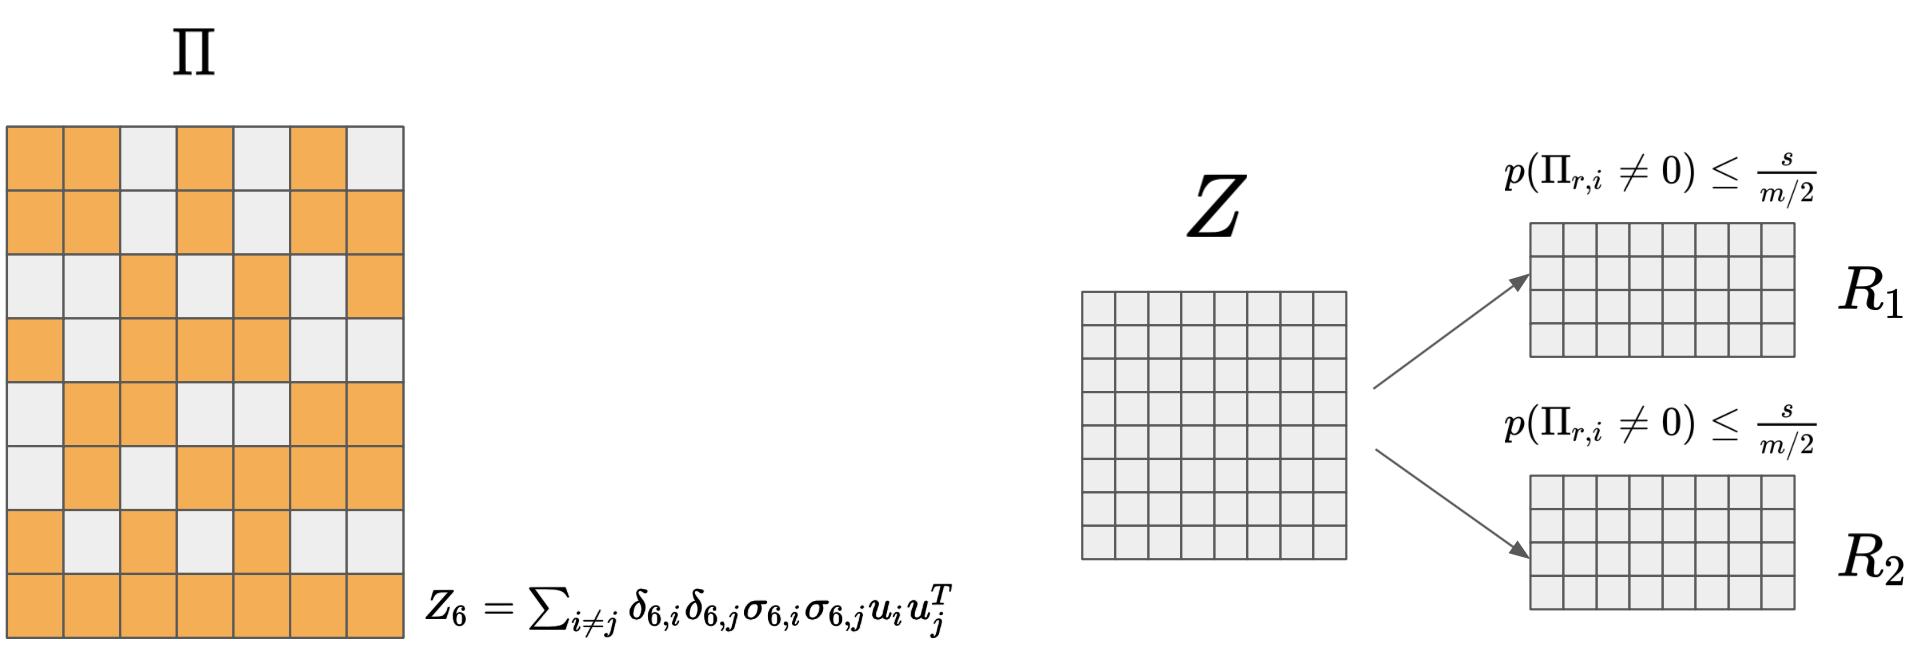
\includegraphics[width=15cm]{figures/splitting.png}
    \caption{Visualization of splitting the matrix to two halves. The orange boxes in matrix $\Pi$ specify the non-zero entries. Here $m = 8$ and $s = 5$. Each column of $\Pi$ has exactly $4$ non-zero entries before the last row.}
    \label{fig:splitting}
\end{figure}

\begin{equation}
    \sum_r Z_r = \sum_{r = 1}^{\frac{m}{2}} Z_r + \sum_{r = \frac{m}{2} + 1}^{m} Z_r = R_1 + R_2
\end{equation}
Even though $R_1$ and $R_2$ are not independent, we can apply Lemma~\ref{lemma_2} to each. The rest of the proof is straightforward. Using the \textsc{Golden-Thompson} lemma and the convexity of the trace, we can find an upper bound for $\av[\tr{\exp(c((\Pi U)^T (\Pi U) - U^TU))}]$ by decomposing it as the contribution of the two halves:
\begin{align*}
    \av[\tr{\exp(c((\Pi U)^T (\Pi U) - U^TU))}]  & \\ 
    &=  \av[\tr{\exp(\frac{c}{s}\sum_{r} Z_r)}] \\
    &= \av[\tr{\exp(\frac{c}{s}(R_1 + R_2))}]  \\ 
    & \leq \av[\tr{\exp(\frac{2c}{s}R_1)}]
\end{align*}
We can show that expected exponential value of the $Z_r$'s in the first half are bounded:
$$
    \av [\exp(\frac{2c}{s} Z_r)] \preceq (2 C^2 d + 1) I
$$
where $\norm{\exp(\frac{4c}{s} x_r {x_r}^{T}) - I } \leq C$ and $x_r = \sum_{i | w_i = 0} \delta_{r, i} \sigma_{r, i} u_i$ and $w_i$'s are $\B$-valued random variables with $P(w_i = 0) = P(w_i = 1) = \frac{1}{2}$. The complete proof for acquiring this bound can be found at~\cite[p6]{cohen2016nearly}.

Now that we have a bound on the expected values of $\exp(\frac{2c}{s} Z_r)$, we can apply Lemma~\ref{lemma_2} on all $Z_r$ variables in $R_1$ where $r \in 1, \dots, \frac{m}{2}$:
\begin{align*}
    \av[\norm{\exp(\frac{2c}{s} Z_r)}] \leq & 2C^2d + 1 \\ \leq & \exp(2C^2 d) \\ 
    \av[\tr{\exp(\frac{2c}{s} R_1)}] \leq & d \exp(C^2dm).
\end{align*}

Therefore,
$$
\av[\tr{\exp(c((\Pi U)^T (\Pi U) - U^TU))}] \leq d \exp(C^2dm).
$$

The following Theorem uses this bound to find the required number of rows $m$ and sparsity $s$ for $\Pi$ to be a subspace embedding. 


\begin{theorem}
    For any $B > 2$, $\delta < \frac{1}{2}$, $\epsilon < \frac{1}{2}$, a sparse embeddings matrix $\Pi$ with $m = O(\frac{Bd\log(d/\delta)}{\epsilon^2})$ and $s = O(\frac{\log_B(d/\delta)}{\epsilon})$ satisfies 
    \begin{equation}
        P(\norm{(\Pi U) ^ T (\Pi U) - U^T U} \leq \epsilon) \geq 1 - \delta
    \end{equation}
\label{main_theorem}
\end{theorem}
\begin{proofsketch}
    It suffices to fix a $c \propto \epsilon^{-1}\log(\frac{d}{\delta})$, such that $s/m \propto \epsilon / Bd$ and $c/s \propto \log B$ and $C^2 d m = 1$. Applying the above lemma to these $c$ and $C$ gives us 
    $$
    \av[\tr{\exp(\epsilon^{-1}\log(d/\delta)((\Pi U)^T (\Pi U) - U^TU) )}] \leq e d.
    $$

Now, we can write
\begin{align*}
        P(\norm{(\Pi U)^T \Pi U - U^TU} \geq \epsilon) & = P(\epsilon^{-1}\log(\frac{d}{\delta}) \norm{(\Pi U)^T \Pi U - U^TU} \geq \log(\frac{d}{\delta})) \\
        & = P(\exp(\epsilon^{-1}\log(\frac{d}{\delta}) \norm{(\Pi U)^T \Pi U - U^TU}) \geq \frac{d}{\delta}) \\
        & = P(\tr{\exp(\epsilon^{-1}\log(\frac{d}{\delta}) ((\Pi U)^T \Pi U - U^TU))} \geq \frac{d}{\delta}) \\
        & \leq \frac{\av[\tr{\exp(\epsilon^{-1}\log(d/\delta)((\Pi U)^T (\Pi U) - U^TU) )}]}{\frac{d}{\delta}} \\
        & \leq \frac{ed}{\frac{d}{\delta}} \\
        & = \calO({\delta})
        \\
          P(\norm{(\Pi U) ^ T (\Pi U) - U^T U} \leq \epsilon) & \geq 1 -  \calO({\delta})
\end{align*}
We can go from the second line to the third line by using lemma~\ref{exp_lemma}, which allows us to bound the spectral norm of the positive semi-definite matrix with its trace. Applying Markov's inequality on line 4 then gives us the desired bound.
 

\end{proofsketch}





\newpage
\bibliographystyle{apalike}
\bibliography{bibs}
\end{document}
